%!TEX root = ../template.tex
%%%%%%%%%%%%%%%%%%%%%%%%%%%%%%%%%%%%%%%%%%%%%%%%%%%%%%%%%%%%%%%%%%%
%% chapter1.tex
%% NOVA thesis document file
%%
%% Chapter with introduction
%%%%%%%%%%%%%%%%%%%%%%%%%%%%%%%%%%%%%%%%%%%%%%%%%%%%%%%%%%%%%%%%%%%
\typeout{NT FILE chapter7.tex}%

\chapter{Application Interface}
\label{chap:ui}

This chapter provides a detailed overview of the application’s user interface. Each page is presented with a description of its structure, components, and functionalities. The pages were designed to be compatible with different browsers, screen sizes, and touch devices. The images shown in this section were taken from a computer. However, certain adaptations have been made to support smaller screens and devices that rely solely on touch interactions. These adaptations will be discussed in the descriptions of the components that were affected.


\section{Main Page}
On the main page (see \autoref{fig:main-page}), the user is presented with a list of available exercises. 

\begin{figure}[h]
    \centering
    \fbox{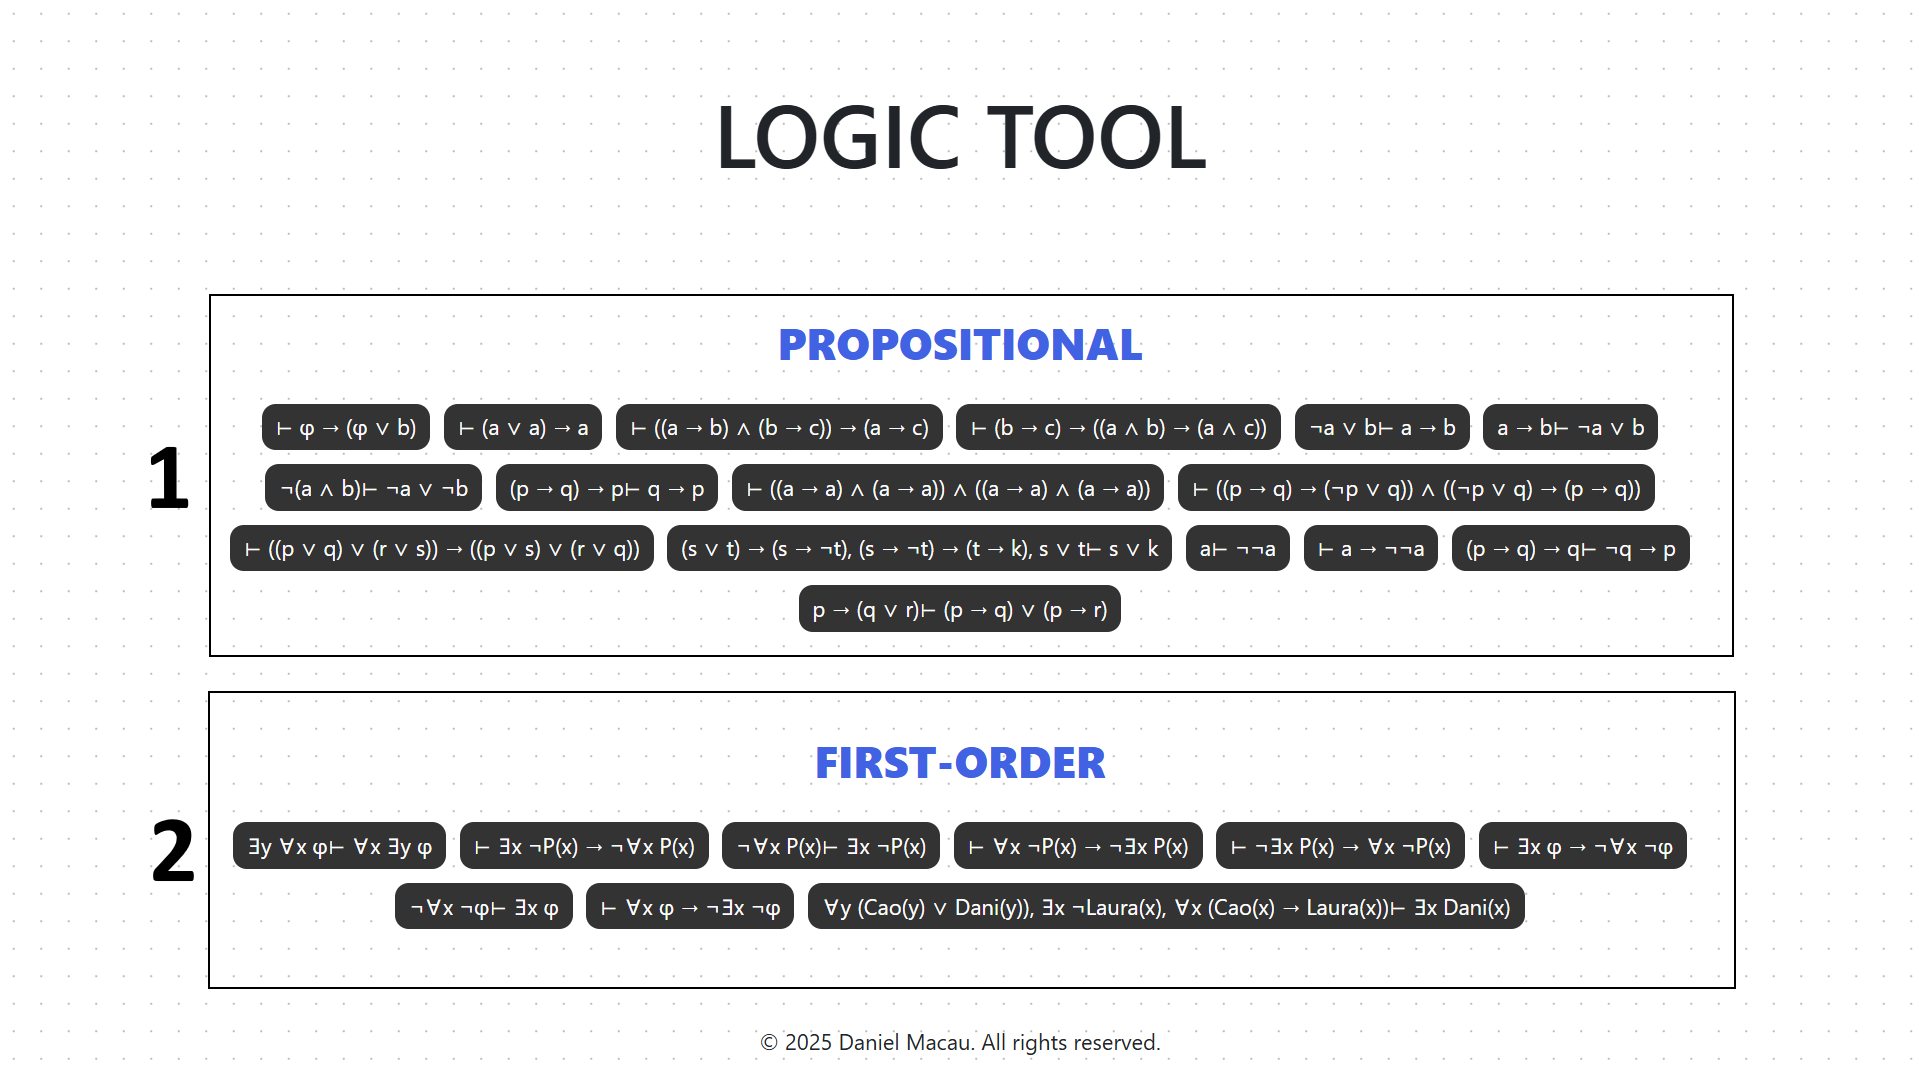
\includegraphics[width=0.95\linewidth]{Chapters/Figures/main-page.png}}
    \caption{Application main page.}
    \label{fig:main-page}
\end{figure}

The list is divided into two categories: \gls{PL} exercises (see item 1 in the figure) and \gls{FOL} exercises (see item 2 in the figure). This separation was a deliberate design choice, as the exercises are based on different logic languages and their difficulty may vary depending on the language used. In a future version, the page could be extended to indicate which exercises have already been completed and which ones are currently in progress. We would also like to add a mechanism allowing users to add new exercises that are not already included in the list of exercises. Additionally, we would like to provide a separate list where users can access the exercises they have saved. Since a session management system has not yet been implemented, these functionalities are currently unavailable.


\section{Board Page}
After selecting an exercise, the user is redirected to the board page (see \autoref{fig:board-page}). 

\begin{figure}[h]
    \centering
    \fbox{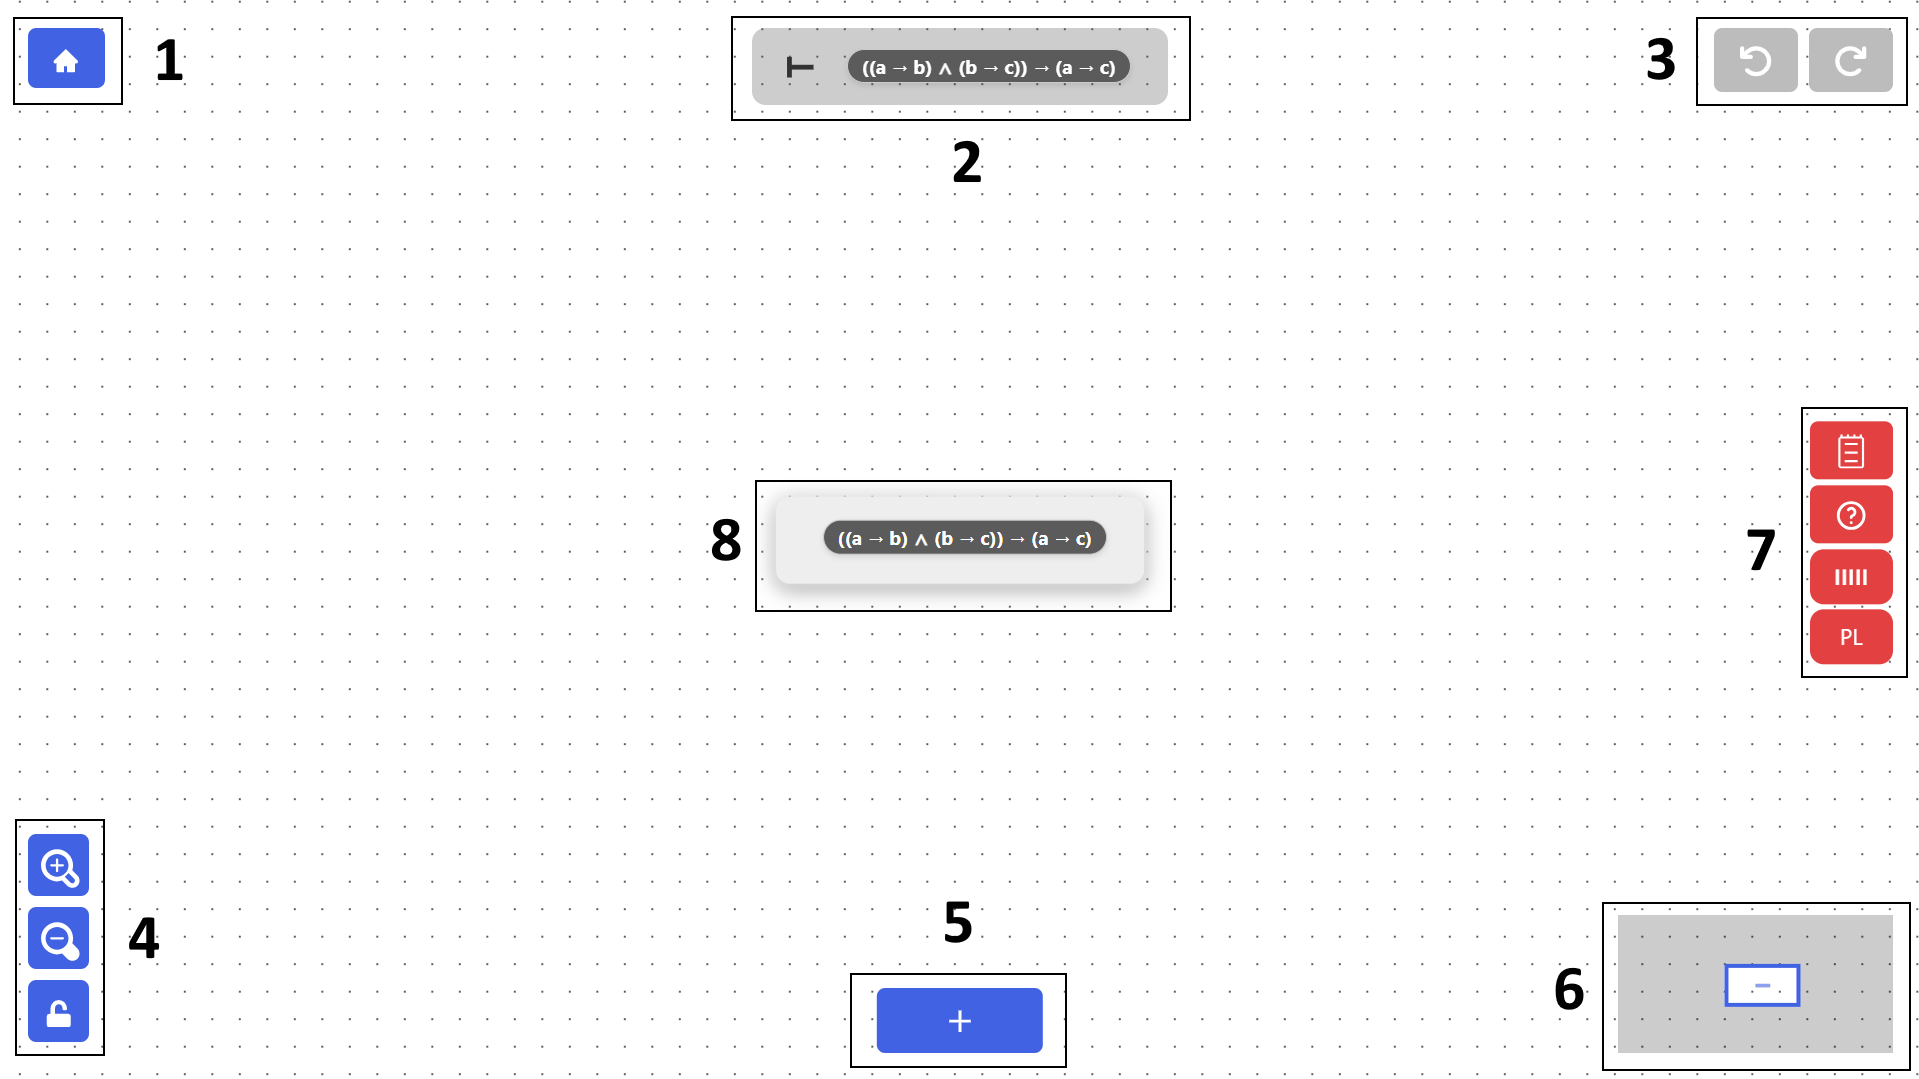
\includegraphics[width=0.9\linewidth]{Chapters/Figures/env-1.png}}
    \caption{Application board page.}
    \label{fig:board-page}
\end{figure}

This page functions as a block-based editor, a visual programming environment, where blocks representing proofs (see item 8 in the figure) can be dragged and dropped onto the board and moved around freely. The choice of a block-based visual editor is based on the way \gls{ND} proofs are usually done on paper. When solving proofs by hand, each step is separate, and we often move between assumptions, conclusions, and sub-proofs. The visual editor tries to map this process by letting users move and arrange proof blocks, showing the logical steps. This makes the transition from paper to the digital environment more intuitive, keeps the step-by-step structure of natural deduction, and enhances the user experience by allowing blocks to be moved freely.

On this page, the user can return to the home page (see item 1) and view the exercise they are currently solving (see item 2). From the exercise statement, users can drag formulas into their proofs, which is especially useful when the exercise includes premises that need to be applied in the construction of the proof. Users can redo and undo their actions (see item 3), zoom in and out, and lock the screen to prevent accidental modifications to the proofs (see item 4). They can also add additional blocks or proofs to the board (see item 5) and visualize them on the map (see item 6). The map displays all blocks present on the board, including overlapping ones, which helps users keep track of components as proofs become larger. Additionally, users have access to the ``dangerous zone'' (see item 7), as it contains operations that could affect learning. They can obtain a complete solution generated by our algorithm, control the amount of feedback they receive by enabling the rules preview or adjusting the level of detail presented in the messages, and also change the logic language they are working with.


\subsection{Blocks (Proofs)}
Now we focus on how the blocks work. As previously mentioned, the board where problems are solved is composed of blocks, which are in fact proofs. The simplest block contains only a formula (represented as 8 in \autoref{fig:board-page}). More complex blocks have rules assigned and can contain multiple formulas, as shown in \autoref{fig:board-blocks}.

\begin{figure}[h]
    \centering
    \fbox{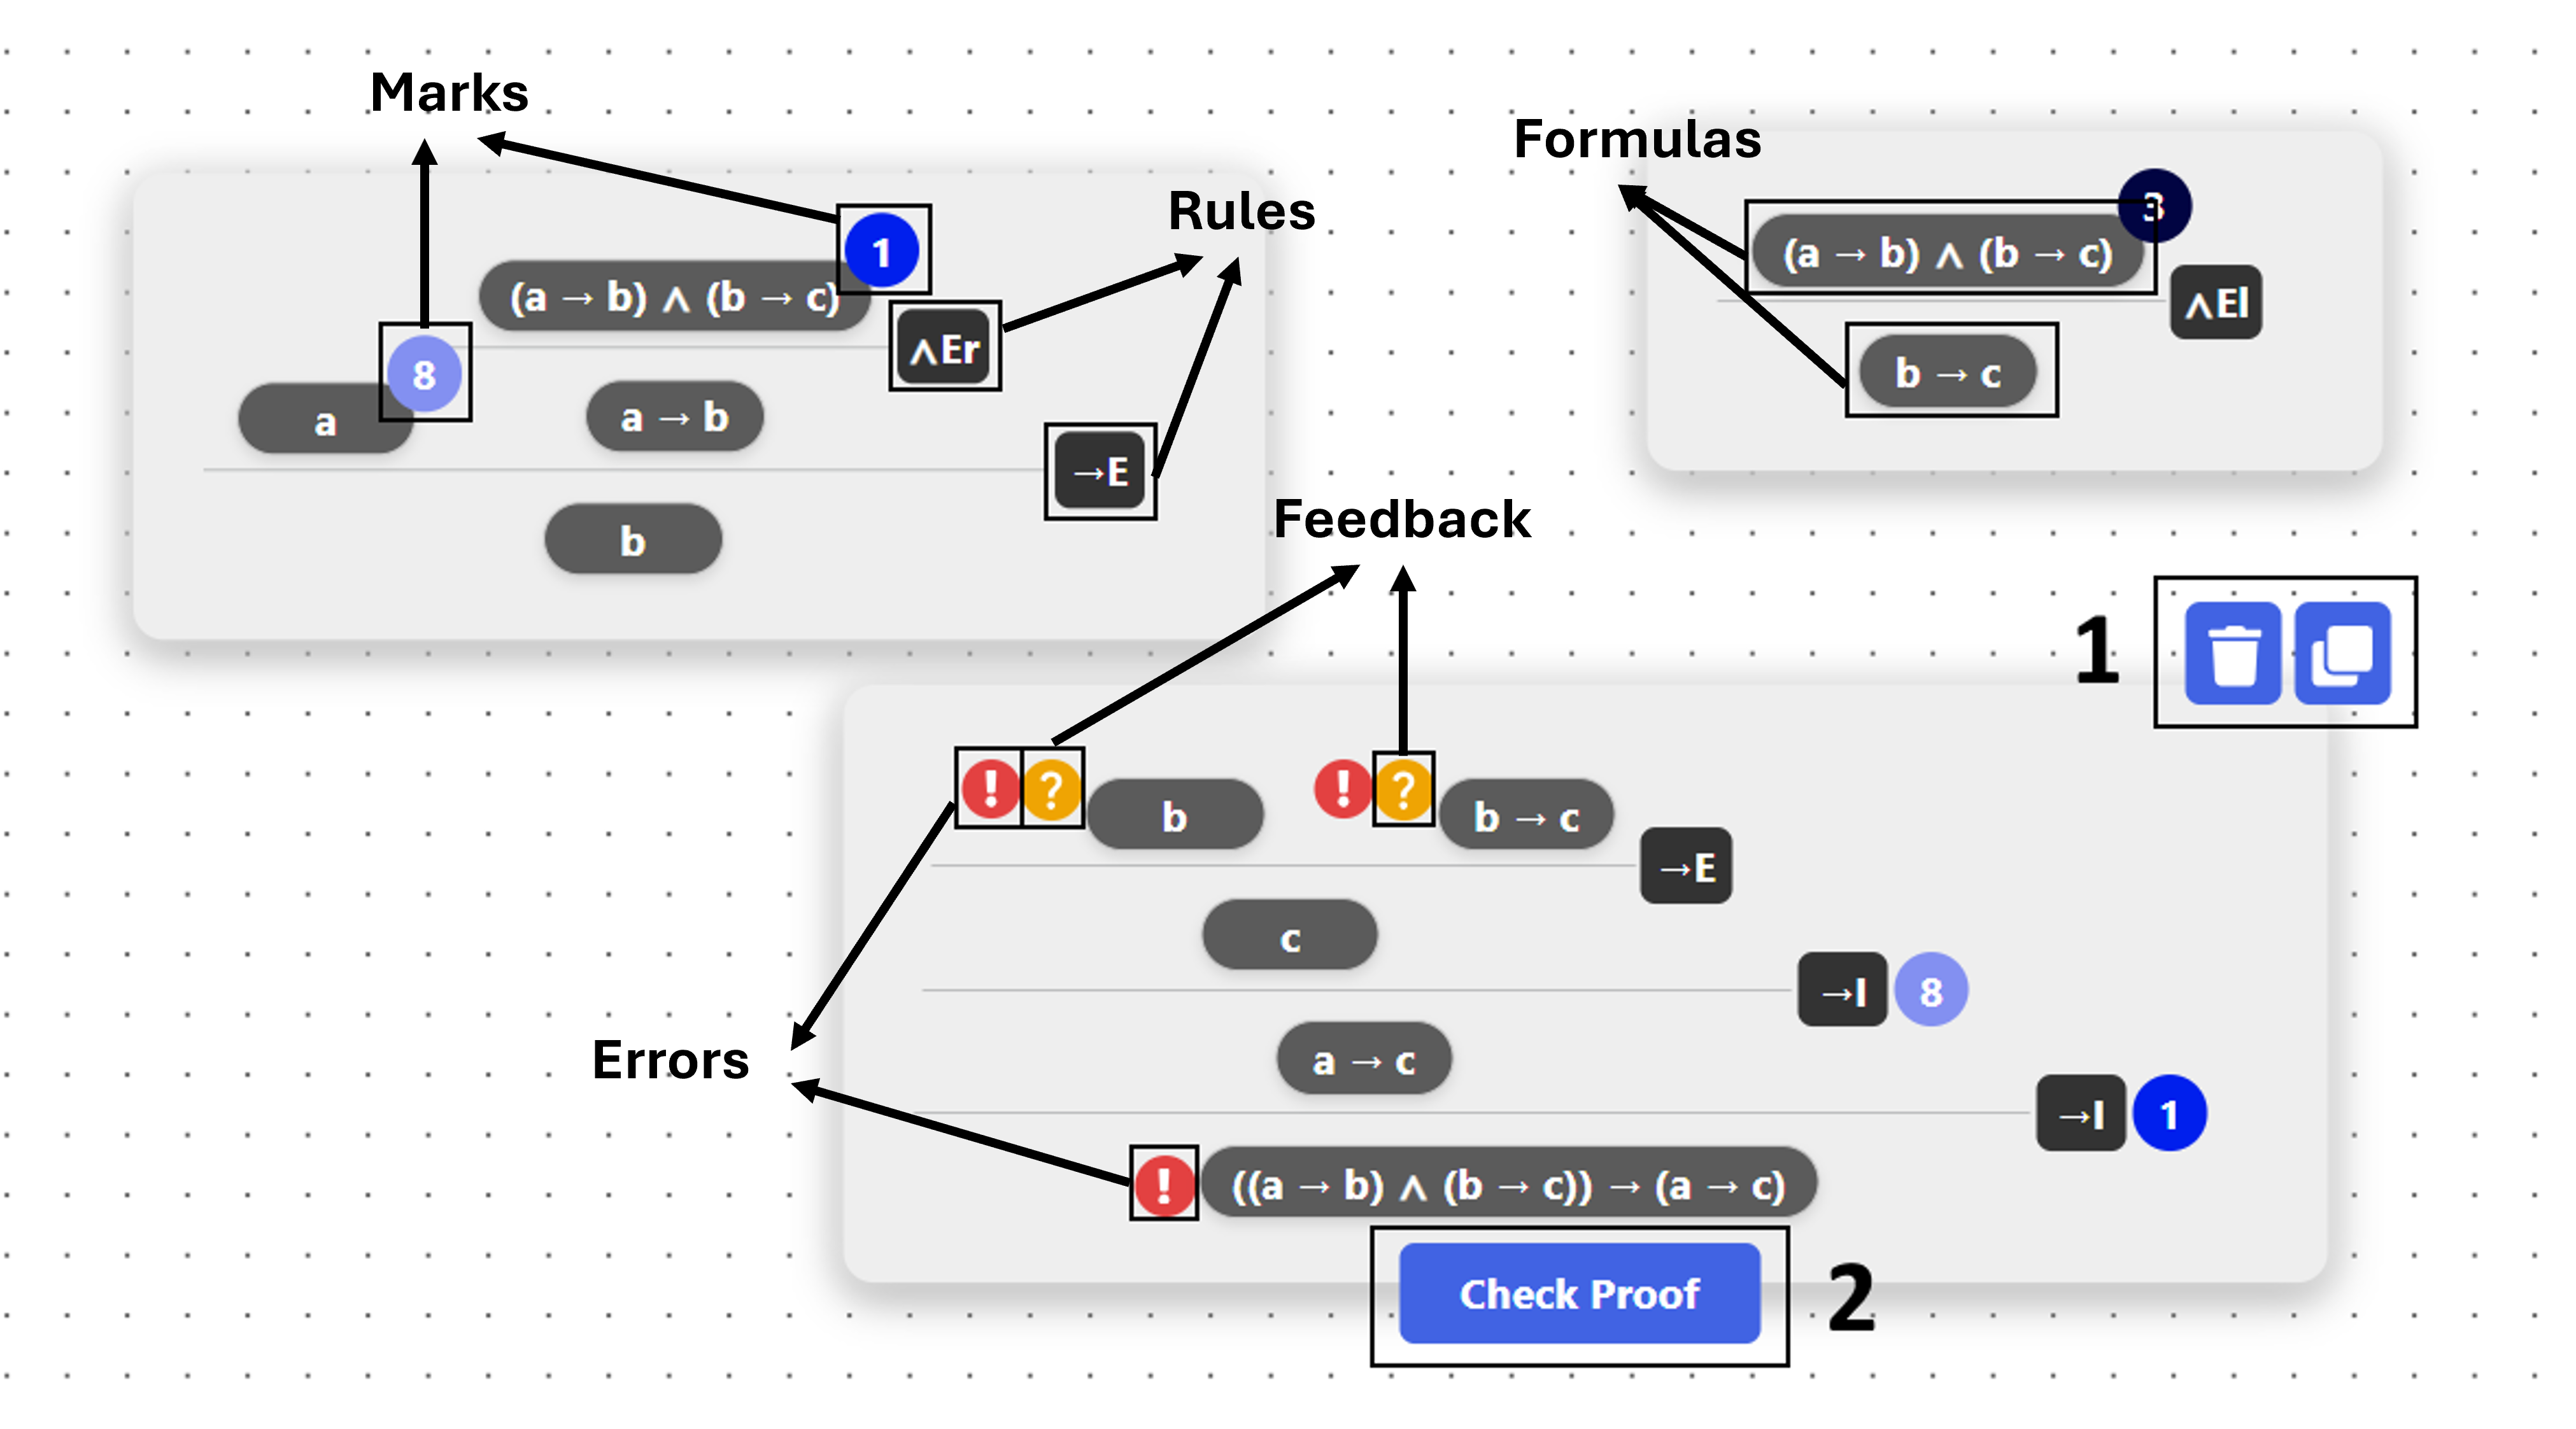
\includegraphics[width=0.95\linewidth]{Chapters/Figures/env-2-2.png}}
    \caption{Application blocks components.}
    \label{fig:board-blocks}
\end{figure}

Complex blocks can be constructed from simpler ones by applying rules or by nesting proofs inside other proofs, which can be done simply by dragging a proof into a formula. Proofs can also be un-nested from other proofs by dragging out the conclusion of the proof that we want to separate.

Each component in a proof is represented with a distinct shape and color: formulas appear as light-gray rounded rectangles, rules as dark-gray squares, and marks in various shades of blue. Rule applications are separated by a horizontal line, similar to their representation on paper. The use of different shapes and colors helps users distinguish between components and understand where each element belongs in the proof. Marks have a flexible coloring system depending on the mark used, which helps students keep track of marks in proofs with many marks. This improves readability, as humans generally detect differences in color more easily than differences in numbers~\cite{color_study}.

Each proof block can be clicked to reveal several options, allowing the user to submit it for checking by the system (see item 2 in the figure), delete it if it is no longer needed, or duplicate it to create a copy (see item 1 in the figure). Once a block is submitted for checking, a message appears at the top if the proof is correct, while in other cases, depending on the feedback level selected, errors and feedback tooltips appear next to formulas or rules. These functionalities will be discussed in more detail in the following sections.

Currently, there are two types of submissions possible. In the first type, if the root of the submitted proof contains the same formula as the conclusion of the exercise, the system checks whether the proof is well-formed and whether it correctly solves the exercise, taking into account the premises of the exercise. We refer to this as the main proof. In \autoref{fig:board-page}, the proof (see item 8) is the main proof, given that we want to prove \(\vdash ((a \to b) \land (b \to c)) \to (a \to c)\). The second type of submission occurs when the root does not match the conclusion. In these cases, the system only checks whether the proof is well-formed. This checking mechanism allows users to validate their sub-proofs before integrating them into the main proof. \autoref{fig:board-submissions} shows the different outputs of the two types of submissions (green boxes).

\begin{figure}[h]
    \centering
    \fbox{%
        \begin{minipage}{\linewidth}
            \centering
            \begin{minipage}[t]{0.59\linewidth}
                \centering
                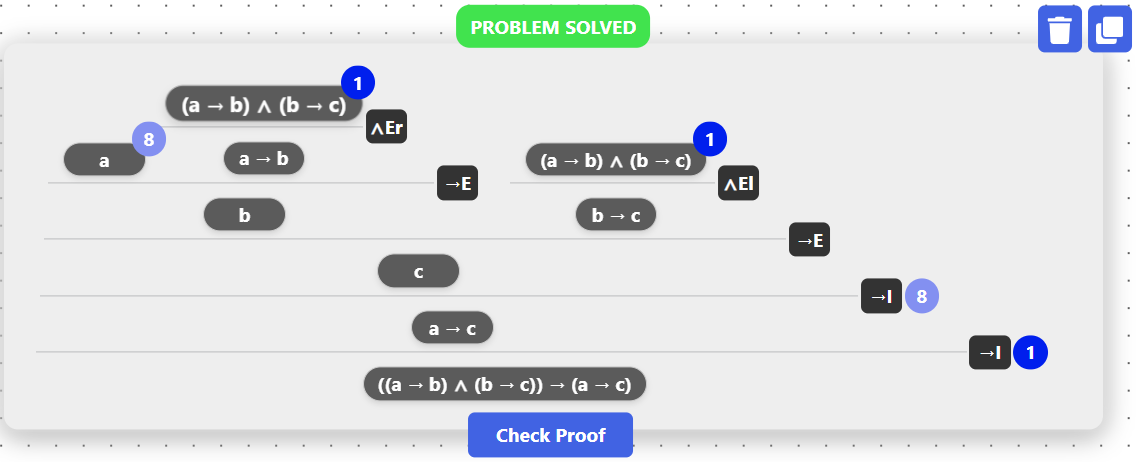
\includegraphics[width=\linewidth]{Chapters/Figures/problem-solved.png}
            \end{minipage}%
            \hfill
            \begin{minipage}[t]{0.39\linewidth}
                \centering
                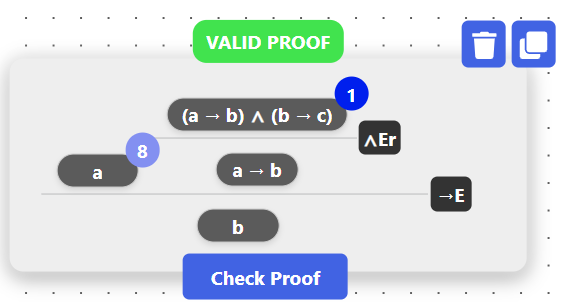
\includegraphics[width=\linewidth]{Chapters/Figures/problem-valid.png}
            \end{minipage}
        \end{minipage}%
    }
    \caption{Application different types of submissions.}
    \label{fig:board-submissions}
\end{figure}

There is a menu that appears when a new rule is added or when an existing rule is changed. This menu lists all the rules available for the logic language currently in use, as shown in \autoref{fig:board-rules}. The menu displays the logic symbols, and by clicking on a symbol the user can access the corresponding rules, including both introduction and elimination rules. When hovering over a rule, a preview is shown that explains how the rule can be applied, following a format similar to the one presented in \autoref{ann:nd_rules}. On touch devices, where hovering is not possible, a tooltip is displayed next to the rule and provides the same preview. In the menu, when clicking on the cross icon, the selected rule is deleted but the sub-proofs that made use of the rule are preserved. This ensures that no work is lost, as illustrated in \autoref{fig:board-rules}.

When a rule is changed, the same process is followed. For example, if the new rule requires fewer hypotheses than the current one, the extra hypotheses are un-nested but preserved as separate blocks, while the remaining ones are kept in the new rule. On the other hand, if the new rule requires more hypotheses, the hypotheses of the old rule are added to the new one.  

\begin{figure}[h]
    \centering
    \begin{minipage}{\linewidth}
        \centering
        \fbox{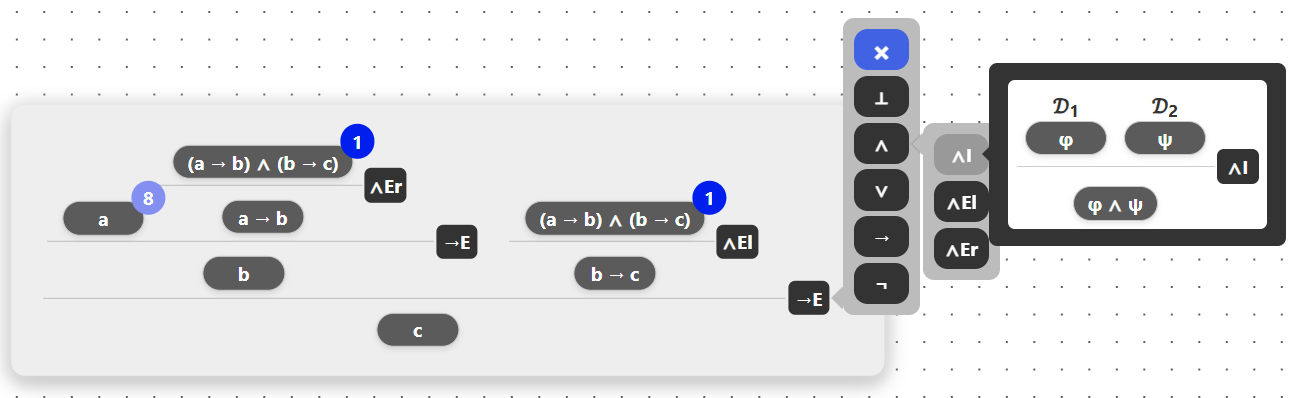
\includegraphics[width=0.85\linewidth]{Chapters/Figures/env-3.png}}\\[0.5em]
        \fbox{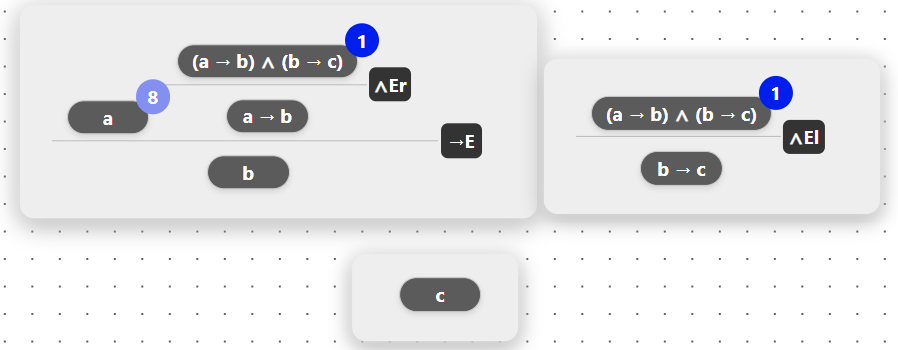
\includegraphics[width=0.85\linewidth]{Chapters/Figures/env-3-3.png}}
    \end{minipage}
    \caption{Rules menu and rule elimination.}
    \label{fig:board-rules}
\end{figure}

For rules that contain predefined formulas, such as negation, and absurdity rules, which all share the formula \(\bot\), the formulas are automatically filled when the rule is applied. In future versions, we plan to extend this mechanism to other rules by using the formulas that have already been inserted, reducing the time required to fill them in manually. However, we do not want this feature to be enabled for all users, since it is also important to practice and memorize how the rules are applied.  

When a user double-clicks on a formula, it enters edit mode, allowing the user to modify the selected formula. Below the formula there is an auxiliary keyboard as shown in \autoref{fig:aux-keyboard}. 

\begin{figure}[h]
    \centering
    \fbox{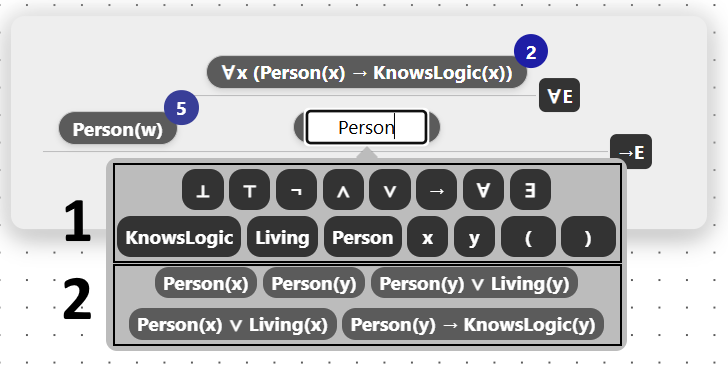
\includegraphics[width=0.7\linewidth]{Chapters/Figures/env-4.png}}
    \caption{Auxiliary keyboard for inserting logical symbols.}
    \label{fig:aux-keyboard}
\end{figure}

This keyboard is extremely useful, as it provides a list of all logic symbols (depending on the current logic language) and the predicates, functions, and variables that are part of the problem being solved (see item 1 in the figure). Additionally, the keyboard includes a filterable list (see item 2 in the figure) of pre-computed formulas derived from the main problem, which updates dynamically as the user modifies the formula or introduces new formulas to the proof. This feature is particularly important for touch-screen devices with small viewports, where switching between virtual keyboards is inconvenient because the operating system's keyboard occupies a large portion of the screen.

For users who prefer to use the normal keyboard instead of the auxiliary one, we follow the common practice and provide a token replacement feature that converts specific words into logical symbols. For example, typing "to" converts to \(\to\), "and" or "\&" converts to \(\land\), and "or" or "|" converts to \(\lor\). The same applies for some Greek letters: "psi" converts to \(\psi\) and "phi" converts to \(\phi\).

When a user clicks on a formula, the system provides options to apply a new rule. If the formula is a leaf, it becomes the conclusion of the new rule. If it is the conclusion of the whole tree, the current tree is used as the first hypothesis of the new rule. \autoref{fig:diff-rules} shows an example of the different rule applications.

\begin{figure}[h]
    \centering
    \fbox{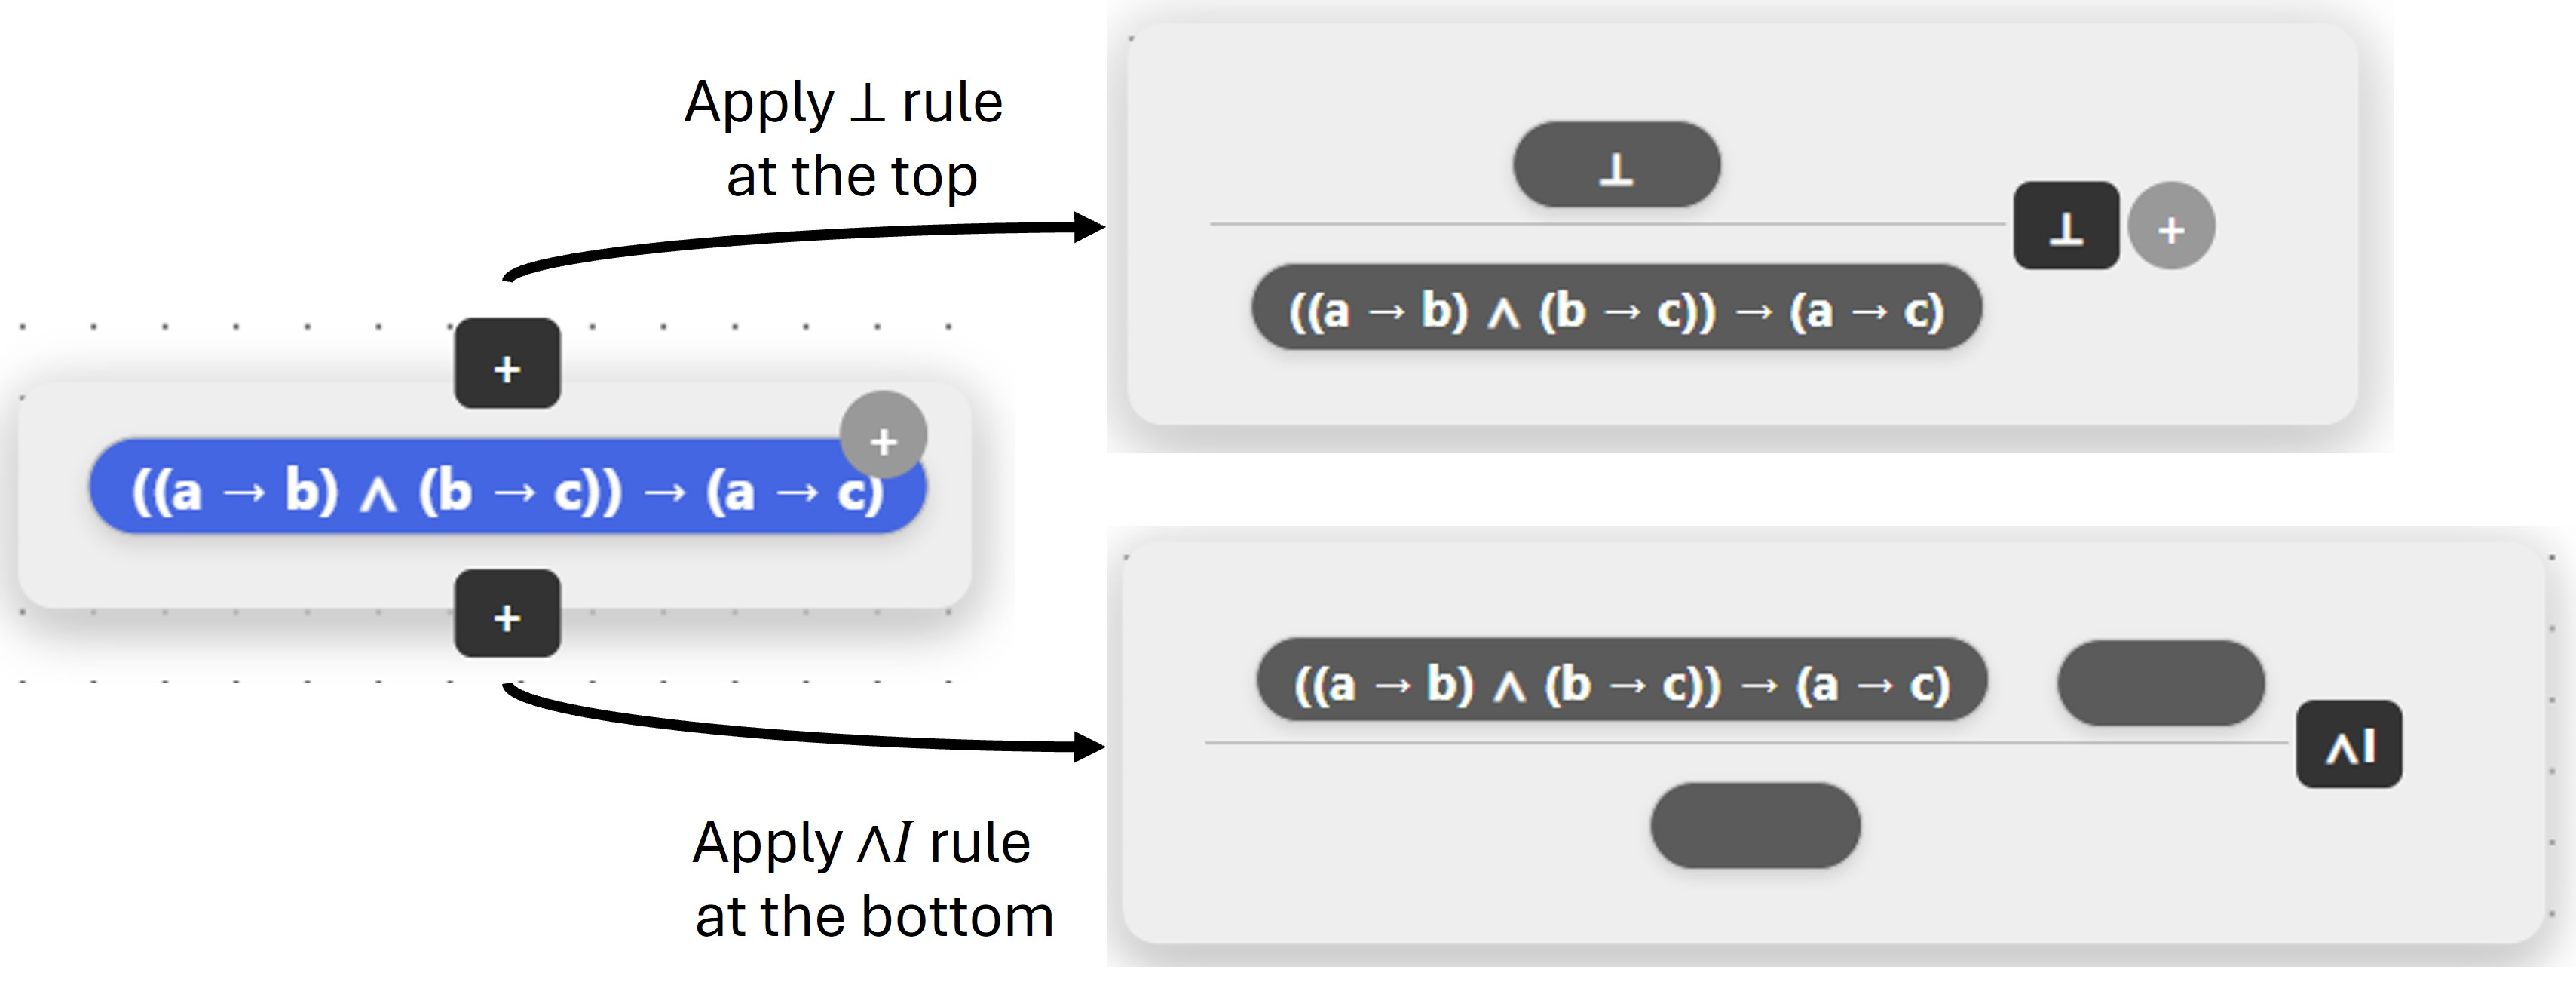
\includegraphics[width=0.95\linewidth]{Chapters/Figures/env-6.jpg}}
    \caption{Different ways to apply a rule to a formula.}
    \label{fig:diff-rules}
\end{figure}

If the formula is a leaf of the proof, a mark can also be assigned to it (see \autoref{fig:menu-marks}).

\begin{figure}[h]
    \centering
    \fbox{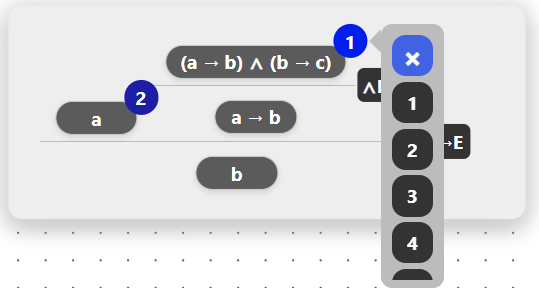
\includegraphics[width=0.6\linewidth]{Chapters/Figures/env-7.png}}
    \caption{Marks menu when clicking on a leaf.}
    \label{fig:menu-marks}
\end{figure}


By clicking on the marks menu, a list of numbers is displayed, which can then be assigned to the current formula. In a future version of the application, we plan to add a mechanism that shows which formulas are assigned to each number when hovering over a mark. This will help students remember the assumptions made up to that point in the proof.

\subsection{Error and Feedback Messages}
Returning to errors and feedback, a submitted proof can contain errors or be incomplete. When this occurs, the tool notifies the user about mistakes and indicates what needs to be corrected. There are different placements for error messages: some occur at the formula level and are independent of the proof, while others are related to the structure of the proof itself. Depending on the selected feedback level, the error messages can provide more detailed information, both regarding the content of the message and the placements of the mistake. Currently, there are five different levels of feedback:  
\begin{itemize}
    \item \textbf{None:} As the name suggests, it does not provide any feedback at all. It only states whether the proof is valid and whether it solves the problem. 
    \item \textbf{Low:} Points out when errors occur in the proof with very generic messages. For example, if the proof does not solve the problem, the user receives the error message: ``This tree does not solve the problem!''.
    \item \textbf{Medium:} Provides more detailed messages, but does not indicate exactly where the error occurred. For example, if a rule has an error, the system reports that the rule is not correctly applied, but does not specify which part of the rule application is incorrect.
    \item \textbf{High:} Specifies where the error occurred, indicating whether it happened in the conclusion or in the premises of a rule application. For example, when a proof is submitted but does not solve the problem, the user receives a message like: ``This tree does not solve the problem! You proved \(\{a\}\vdash (a \lor a) \to a\)'' where the goal was to prove \(\vdash (a \lor a) \to a\).
    \item \textbf{Solution:} The highest level of feedback. It points out the error to the user and, if possible, provides a suggestion on how to solve the problem by showing an alternative solution.
\end{itemize}

\subsubsection*{Formula-level errors:}
Below, we list some errors that occur when a user enters a formula with errors.

\vspace{1em}
In this first example, the user inserted the character ``\$'', which is not a valid symbol in logic. At the Medium feedback level, the user receives a generic message indicating a lexical error, but it did not specify the error in detail.

\begin{center}
\fbox{
\includegraphics[width=0.35\textwidth]{Chapters/Figures/error-1.png}}
\end{center}

In this example, the user inserted two literals without a logic symbol separating them, which is not valid. At the High feedback level, the error message indicated that a logical symbol was expected between the two literals.

\begin{center}
\fbox{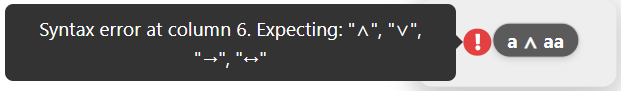
\includegraphics[width=0.58\textwidth]{Chapters/Figures/error-2.png}}
\end{center}

In this example, the user forgot to close the parenthesis. At the Solution feedback level, the system provides the solution, instructing the user to close the parentheses at the end of the formula.

\begin{center}
\fbox{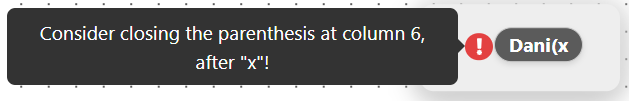
\includegraphics[width=0.58\textwidth]{Chapters/Figures/error-3.png}}
\end{center}

In this example, the user forgot to assign a variable to the quantifier. At the High feedback level, the system warns the user that a variable is missing after the quantifier and specifies the column in which the error occurs.

\begin{center}
\fbox{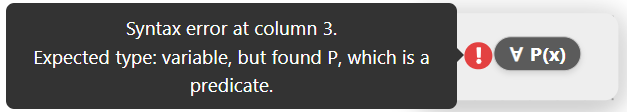
\includegraphics[width=0.58\textwidth]{Chapters/Figures/error-4.png}}
\end{center}

In this example, the user forgot to add parentheses to the expression to resolve ambiguities. At the Solution feedback level, the system instructs the user to surround the expression \(a \land a\) with parentheses to eliminate the ambiguity.

\begin{center}
\fbox{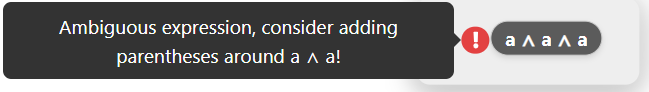
\includegraphics[width=0.58\textwidth]{Chapters/Figures/error-5.png}}
\end{center}

In this final example, the user called the same predicate with two different arities. At the High feedback level, the system informs the user that the predicate \(Living\) was used with two arguments instead of one.
\begin{center}
\fbox{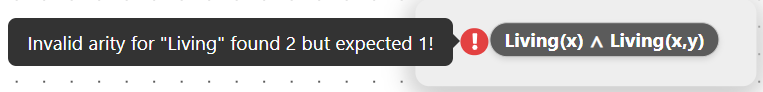
\includegraphics[width=0.58\textwidth]{Chapters/Figures/error-7.png}}
\end{center}

\subsubsection*{Proof-level errors:}
Focusing on proof-level errors, the application guarantees that lexical and syntactic errors cannot occur during proof construction. This guarantee is ensured by the way proofs are created and submitted. For instance, when a user adds a rule to a proof, the system automatically enforces the correct number of hypotheses and marks required by that rule. Similarly, the application ensures that every formula within a proof is properly filled before submission. By controlling these aspects during proof construction, the system prevents any malformed formulas or structural violations, effectively eliminating syntactic errors at the proof level. As a result, only semantic errors are shown to users. Below, we list some errors that occur when a user tries to prove a problem.

\vspace{1em}

In this first example, we illustrate a problem where the user forgot to assign a mark to one of the leaves of the tree. On the left, the error is presented to the user at a High feedback level, listing all available marks that can be used at that stage of the proof and allowing the user to decide what to do next. On the right, the feedback is at the Solution level, where the system clearly indicates the correct action: the user should assign the mark one to the formula.

\begin{center}
\fbox{%
  \begin{minipage}{0.45\textwidth}
    \centering
    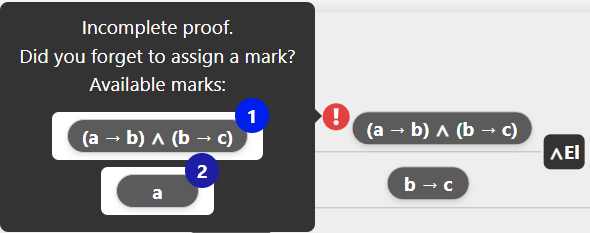
\includegraphics[width=\linewidth]{Chapters/Figures/error-8.png}
  \end{minipage}%
  \hspace{0.02\textwidth}
  \begin{minipage}{0.48\textwidth}
    \centering
    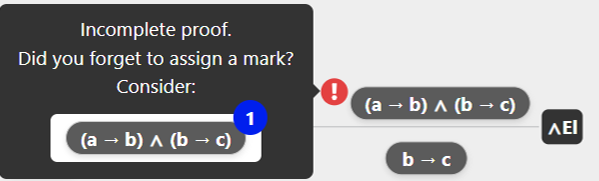
\includegraphics[width=\linewidth]{Chapters/Figures/error-9.png}
  \end{minipage}%
}
\end{center}

In this example, the user applied the \(\forall_I\) rule incorrectly because the mapping between the variables is wrong. At the Solution feedback level, the system can find a solution and presents it in a tree, as shown in the first image. At the High feedback level, the system identifies which part of the proof is incorrect, as shown in the second image, and explains exactly what is wrong. In this case, the variable mapping is incorrect.

\begin{center}
\fbox{%
  \begin{minipage}{0.58\textwidth}
    \centering
    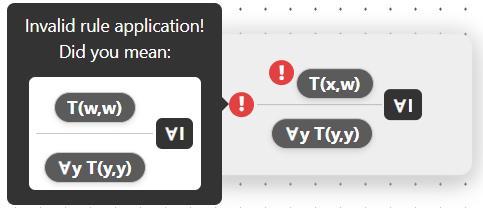
\includegraphics[width=\linewidth]{Chapters/Figures/error-10.png}
    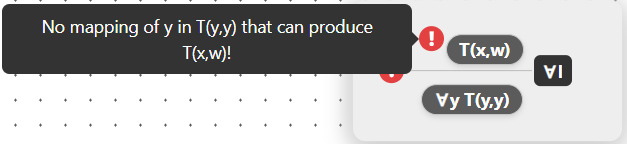
\includegraphics[width=\linewidth]{Chapters/Figures/error-11.png}
  \end{minipage}%
}
\end{center}

In this example, the user solved the wrong problem. Instead of solving \(\vdash (a \lor a) \to a\), they solved \(\{a\} \vdash (a \lor a) \to a\). The system clearly indicates which problem was solved. In fact, it detects the extra hypothesis that prevents the user from solving the correct problem. If the user hovers over the error on that hypothesis, a feedback message similar to the one in the first example of proof errors will be shown.
\begin{center}
\fbox{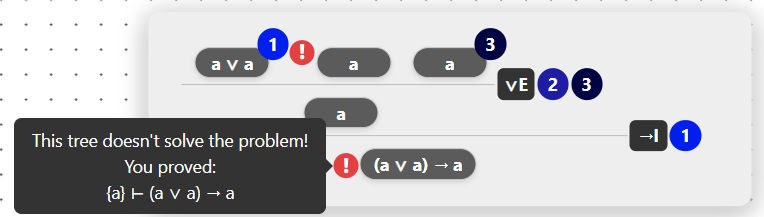
\includegraphics[width=0.58\textwidth]{Chapters/Figures/error-12.png}}
\end{center}

\subsection{Proof feedback/hints:}
In addition to detecting errors, the system can identify when a proof is incomplete and provide feedback to guide the user on how to proceed. This type of feedback is enabled by the algorithm we developed, which can automatically solve \gls{ND} proofs (see \autoref{chap:algo}). Below, we list some types of messages that users can receive when they do not know how to proceed.

\vspace{1em}
In these examples, the user is stuck at \(p\) and does not know what to do next. In the left image, the feedback level is set to Solution, providing the concrete step that the user should apply to complete the proof. In this case, the user should apply the \(\to_E\) rule. In the right image, the feedback level is set to Medium, so the hint given to the user is more generic and indicates that they need to apply two more rules to solve the problem. 

In Solution mode, we could show a proof with the correct formulas already filled in for the rule application. However, we decided not to do this because it would give too much information, and students might stop thinking on their own and rely only on the hints from the system.

\begin{center}
\fbox{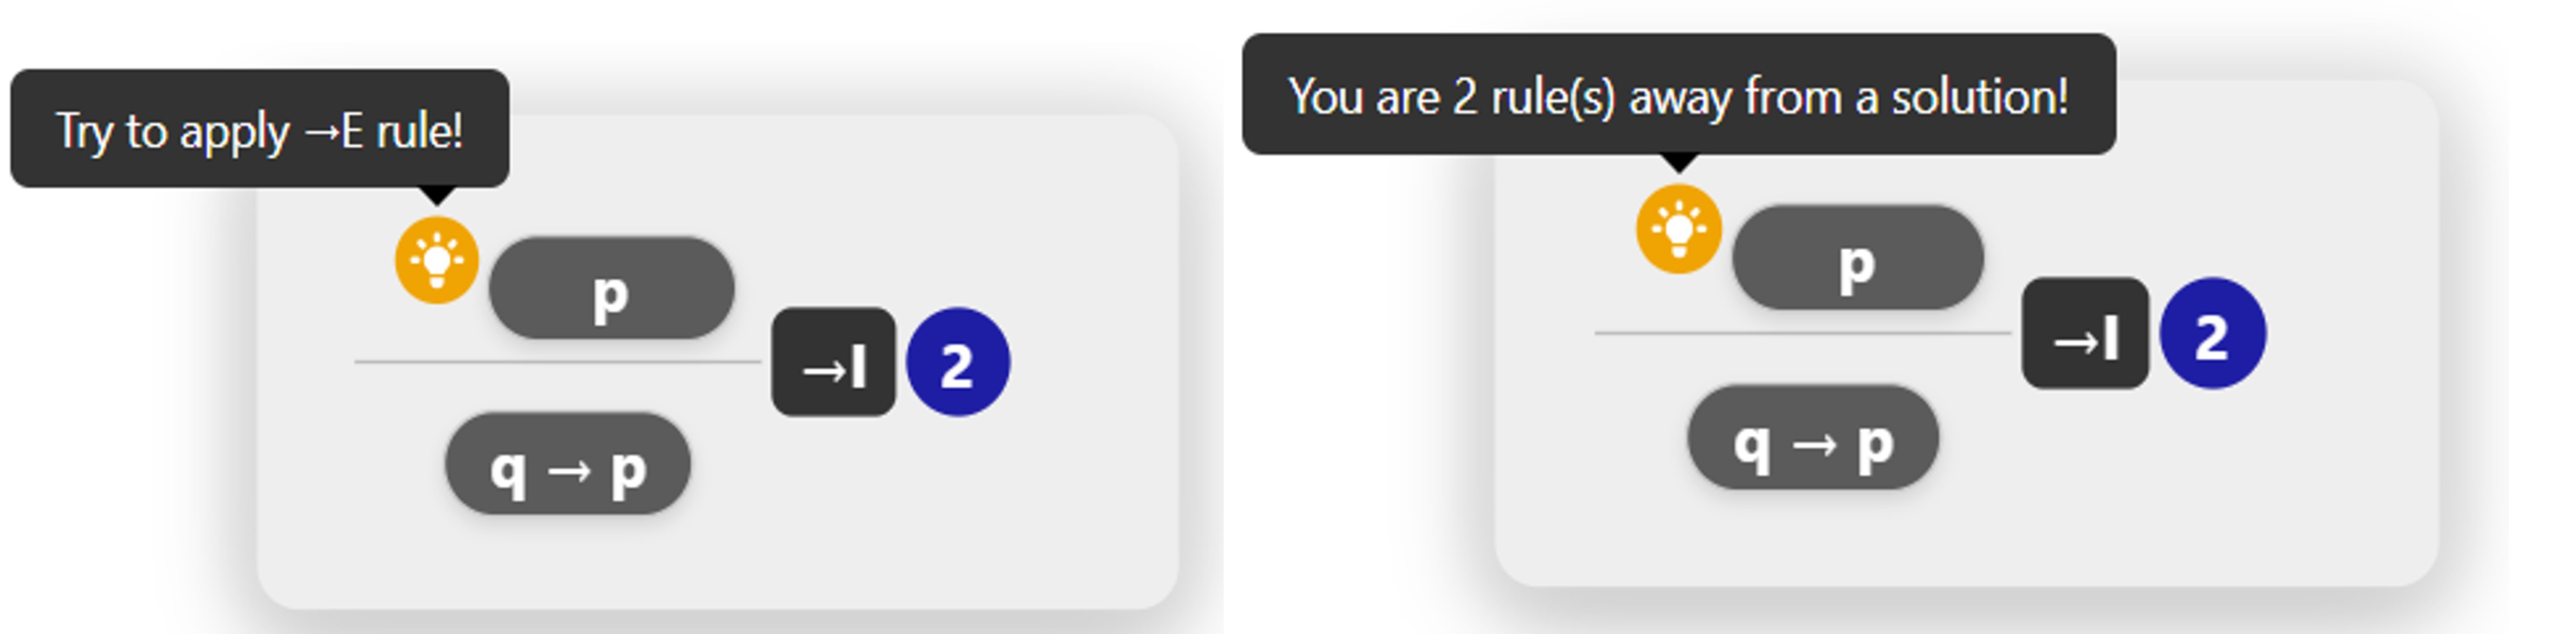
\includegraphics[width=0.95\linewidth]{Chapters/Figures/proof_feedback.jpg}}
\end{center}

\subsection{Other features}

There are several other features designed to improve the interactivity and usability of the tool. For instance, when a user starts dragging a proof, the system highlights, through animations, the locations where the proof can be placed, making it easier to understand where it can go. Similarly, when a user requests feedback, the server may take some time to process the request, especially if it involves running a complex algorithm. In these cases, a loading animation is displayed to indicate that the system is processing the request.

Moreover, the tool supports many shortcuts that allow users to work more efficiently and quickly when constructing proofs. For example, users can select a proof and copy or paste it using \texttt{CONTROL+C} and \texttt{CONTROL+V}. Proofs, formulas, rules, or marks can be deleted simply by selecting them and pressing the \texttt{Delete} key. Undo and redo operations are also supported using \texttt{CONTROL+Z} and \texttt{CONTROL+Y}, respectively.